\chapter{FUNDAMENTALS}\label{chapter:fundamentals}

In this chapter, we are going to define the basic concepts needed to understand the contents of this paper.
The mathematical details of algorithms or technical implementations of the presented technologies will not be described in depth, but rather briefly and concisely describe how they work.

@isenko: still working on this part!

We will formally define what are neural networks and how training works using a simple scenario.
Following, we will introduce why and how distributed computing techniques are important in today's world, and how they can be used to facilitate neural network training.
The topic of distributed neural network training is then presented.
Finally, we describe Hivemind, how it works, why we chose this framework, which type of analysis we are going to conduct, and what kind of parameters are we focusing on in this paper.

\section{Neural Networks}
Neural networks (NNs) have been a major research area in the past decade.
However, the basics of NNs as we know them today have been around for almost 70 years but did not gain much recognition until the 2010s.
This is mostly because the success and viability of NNs are affected by two major factors, data availability and computational power, both of which were scarce or not advanced enough.
As network-connected devices like smartphones and laptops started to become more widespread, the data that could be generated and gathered grew by several orders of magnitude.
Today, NNs are used in many fields, from pharmaceutical to translation, from art generation to autonomous driving.

Let us introduce a simple example to support the following explanations.
We might want to classify many images of cats and dogs using a NN so that its inputs are images of cats or dogs, and the output is a binary variable indicating $0$ if the image is a cat and $1$ if it is a dog.

To understand NNs, we have to look at their smallest components called \textit{neurons}, which are functions that can be defined as follows:
\begin{equation}
    y = g(X \cdot W + b)
\end{equation}
where $g$ is called the activation function, $X \in \mathbb{R}^n$ is the neuron's input, $y \in \mathbb{R}$ is the output, $W \in \mathbb{R}^n$ its weights or parameters, and $b \in \mathbb{R}$ its bias.
Note that activation functions must be non-linear functions.
We would like to use NNs to solve and predict non-linear problems such as our example, a task that can only be achieved by using non-linear functions.
If we were to compose a neural network using only linear functions, the output would still be a linear function, regardless of a NN's complexity.
Examples of non-linear functions commonly used inside NNs are the sigmoid and the rectified linear unit (ReLU).
The weights $W$ and the bias $b$ define the result of the activation function $g$.

The first and most simple type of NN that was devised is called \textit{feed-forward neural network} (FF) and is comprised of many neurons stacked together in \textit{layers}.
These layers $f$ are then composed together to form a feed-forward NN:
\begin{equation}
    Y = f_1 \circ f2 \circ \ldots \circ f_L
\end{equation}
where $L$ is called the \textit{depth} of a FF neural network, or number of \textit{hidden layers} in a FF network.

\begin{figure}[h]
    \centering
    \caption{An example of a neural network, with input layers (green nodes), hidden layers (blue nodes), and output layer (red node).}
    \label{fig:neural-network}
    
\begin{tikzpicture}[x=2.2cm,y=1.4cm]
    \message{^^JNeural network without arrows}
    \readlist\Nnod{2,3,3,3,1} % array of number of nodes per layer
    
    \message{^^J  Layer}
    \foreachitem \N \in \Nnod{ % loop over layers
      \def\lay{\Ncnt} % alias of index of current layer
      \pgfmathsetmacro\prev{int(\Ncnt-1)} % number of previous layer
      \message{\lay,}
      \foreach \i [evaluate={\y=\N/2-\i; \x=\lay; \n=\nstyle;}] in {1,...,\N}{ % loop over nodes
        
        % NODES
        \node[node \n] (N\lay-\i) at (\x,\y) {$a_\i^{(\Ncnt)}$};
        
        % CONNECTIONS
        \ifnum\lay>1 % connect to previous layer
          \foreach \j in {1,...,\Nnod[\prev]}{ % loop over nodes in previous layer
            \draw[connect,white,line width=1.2] (N\prev-\j) -- (N\lay-\i);
            \draw[connect] (N\prev-\j) -- (N\lay-\i);
            %\draw[connect] (N\prev-\j.0) -- (N\lay-\i.180); % connect to left
          }
        \fi % else: nothing to connect first layer
        
      }
    }
    
    % LABELS
    \node[above=5,align=center,mygreen!60!black] at (N1-1.90) {input\\[-0.2em]layer};
    \node[above=2,align=center,myblue!60!black] at (N3-1.90) {hidden layers};
    \node[above=8,align=center,myred!60!black] at (N\Nnodlen-1.90) {output\\[-0.2em]layer};
    
  \end{tikzpicture}
\end{figure}

The depth, as well as the types of layers and functions of a given neural network, define its \textit{architecture}.
A NN architecture can be changed to obtain different results in terms of effectiveness, speed or other criteria.
An example of one such architecture is represented in \autoref{fig:neural-network}.

At this point, the model has fixed parameters $W$ and $b$, so given the same input, the output will be the same.
We would like to update the parameters in such a way that the output reflects some arbitrary characteristic of the input, a process called \textit{training}.

\subsection{Training}

Using our example, the NN should learn over time and using many examples, which images represent a cat, and which ones represent a dog.
We can provide information to the neural network about whether or not it is right or wrong, and update its parameters according to how much it is far from the truth.

Formally, the function determining how much a NN is wrong about a guess is called a \textit{loss function}, which outputs a value called \textit{loss}.
For a binary value such as our example, we can use the \textit{binary cross entropy} loss function.
The lower this value is, the closest the NN is to the ground truth.

We can derive certain properties from this value, such as how much should we change the parameters of our NN model so that we get a lower value the next time we try.
This approach can be formally described as an optimization problem, where the optimization function, also called optimizer, is defined as follows:
\begin{equation}
    \arg \min_{W, b} \mathcal{L} (W, b)
\end{equation}

The optimizer function defines how the values of $W$ and $b$ should change to get a better loss.
The process of iteratively updating these values multiple times using different inputs is called \textit{training}.
Commonly used optimizers for NN training are \textit{Stochastic Gradient Descent}, \textit{Root Mean Square} (RMSProp), \textit{Adam} and others.

The values obtained using these optimization functions are used to determine the best next local optima for the given parameters.
This process can then be repeated multiple times until an arbitrary loss value is reached, and the training process is stopped.
The final architecture of the neural network and the state of the weights and biases are then fixed, obtaining the final NN model.

At several stages during training, a neural network practitioner might want to validate the results obtained by using a set of data that is different from the one that has been used to train the NN.
This is called the \textit{validation step}, and it is performed without changing the network's parameters or architecture.
Validation steps are crucial to understanding if the changes made to a model are biased towards a specific set of inputs, an effect denominated \textit{underfitting}.

\subsection{Gradient Accumulation}\label{sec:gradient-accumulation}

When training neural networks, increasing batch size can sometimes lead to faster convergence \cite{Krizhevsky2014owt, goyal2017accurate, you2017scaling}.
However, simply increasing the batch size during training does not scale very well, and can lead to memory issues or an inability to train at all.
To help simulate bigger batches on a single device without incurring these issues, we can use a technique called \textit{gradient accumulation}.

Algorithm~\ref{alg:standard-training} shows a simplified version of an algorithm used to train neural networks.
A dataset consisting of a set of inputs $X$ and $Y$ labels, both with length $N$, is used as the input to the model, with a training loop supporting a single epoch.


\begin{algorithm}
    \caption{Standard training algorithm, PyTorch style}\label{alg:standard-training}
    \begin{algorithmic}
        \Require $N \geq 0$
        \State $X \gets [...]$ \Comment{Inputs}
        \State $Y \gets [...]$ \Comment{Labels}
        \State $i \gets 0$
        \While{$i < N$}
        \State $prediction \gets model(X[i])$
        \State $loss \gets $ criterion$(prediction, Y[i])$
        \State $loss$.backward()
        \State optimizer.step()
        \State optimizer.zero\_grad()
        \State $i \gets i + 1$
        \EndWhile
    \end{algorithmic}
\end{algorithm}

Algorithm~\ref{alg:grad-acc-training} shows a modified version of Algorithm~\ref{alg:standard-training} with gradient accumulation turned on.
This technique introduces an accumulation variable ($ACC$) instructing how many batches should be accumulated within the optimizer's state.
The $loss$ value is normalized with the value of $ACC$ to account for the effects of the accumulation.
Once $ACC$ batches have been aggregated or when we have finished training, we apply the averaged gradients using the optimizer's function $optimizer.step()$, and reset its gradients to zero.

\begin{algorithm}
    \caption{Training with gradient accumulation, PyTorch style}\label{alg:grad-acc-training}
    \begin{algorithmic}
        \Require $N \geq 0$
        \Require $ACC > 0$
        \State $X \gets [...]$ \Comment{Inputs}
        \State $Y \gets [...]$ \Comment{Labels}
        \State $i \gets 0$
        \While{$i < N$}
        \State $prediction \gets model(X[i])$
        \State $loss \gets $ criterion$(prediction, Y[i])$
        \State $loss$.backward()
        \State $loss \gets loss / ACC$
        \If{$((i + 1) \mod{ACC} == 0)$ or $((i + 1) == N)$}
        \State optimizer.step()
        \State optimizer.zero\_grad()
        \EndIf
        \State $i \gets i + 1$
        \EndWhile
    \end{algorithmic}
\end{algorithm}

\section{Distributed Computing and Storage for Neural Networks}

A distributed system is defined as a system where its components communicate with one another using messages.
In computer science, the use of distributed systems has been a field of research for many years and has boomed with the advent of network communications.
We often see distributed systems in complex applications such as the backend of a website or supercomputers.
These systems are often composed of tens or hundreds of connected components that collectively produce one or more outcomes, such as web pages or complicated simulations.
Using distributed techniques is essential for these complex applications, as the computational load and complexity required to run them, are simply too great for a single machine.

The elevated number of components that make a distributed system can lead to several issues, such as an immense amount of requests to their local storage and extremely large files.
For these reasons, it is necessary to use storage solutions that can handle these kinds of stress.
Several distributed storage solutions have been developed and adopted over the past years, each of them excelling in different solutions and lacking in other areas.
In general, choosing the right distributed storage software is crucial, as it can mean the difference between loading a dataset in seconds or minutes.

Neural networks have quickly become too large in terms of memory and computationally expensive for a single host, thus needing distributed system techniques for training.

\section{Distributed Training}
Training a state-of-the-art neural network nowadays requires enormous amounts of time and effort, but especially resources and money.
It is often impossible to train a model within the boundaries of a single piece of hardware, even with powerful specifications.
This affects the speed at which neural networks are being developed and the ability to reproduce results from state-of-the-art models.

One of the first and most notable examples of the results of this phenomenon is AlexNet \cite{alexnet2012}, in which the authors mentioned the need of using more than one GPU to train their model.
This was 2010, and a little more than a decade later, to train the newest neural network models, practitioners, companies and research institutes need thousands of powerful GPUs.
Distributed system techniques are used to be able to train these massive neural networks, creating the new term ``distributed training''.

We briefly summarize distributed training techniques as follows:
\begin{itemize}
    \item \textbf{Data parallelism};
          given a set of $n$ devices, an instance of the model is trained on each one of the devices.
          Usually, gradients obtained during backpropagation are then aggregated across all the devices using techniques such as \textit{AllReduce}.
          This technique however does not work very well with models that exceed a single device's available memory and is therefore used in applications with low-memory devices such as \textit{Federated Learning} \cite{li2019federatedlearning}.

    \item \textbf{Model parallelism};
          a deep neural network is conceptually split into $n$ partitions across $n$ devices, each hosting a different partition and set of weights.
          An early notable example of model parallelism is AlexNet \cite{alexnet2012}, where the authors decided to split the computation of some of the layers across two GPUs with 3GB of ram each, a concept illustrated in \autoref{fig:alexnet}.
          This technique relieves the burden of a single node to host all of the weights of a model but is also more sensitive to issues with communication across nodes.

    \item \textbf{Pipeline parallelism};
          a combination between model parallelism and data parallelism.
          Pipeline parallelism for machine learning models has been introduced in 2018 \cite{huang2018gpipe}.
          With this technique, each batch is split into micro-batches and sent to available computing devices such as GPUs, which individually compute both the forward and backward pass for that micro-batch.
          Finally, weights are averaged after backpropagation has taken place on every GPU.

    \item \textbf{Tensor parallelism};
          tensor operations for huge neural network models can become a bottleneck, as they can require more memory than the host's device can handle and can become slow in general.
          Tensor parallelism can alleviate a single node's computational burden by splitting a tensor operation across many devices.
          This technique has been first introduced in neural network models in \cite{dean2012distbelief} with a framework called DistBelief.

    \item \textbf{Mixture-of-Experts}.
          Instead of conceptually splitting a model, we construct multiple, different models and split them across workers, also called ``experts''.
          A gating function helps each of the experts to specialize in a different subset of all training cases.
          The broader concept has been first introduced in 1991 \cite{Jacobs1991mixtureofexperts} but has recently gained traction due to its flexibility in solving natural language problems.
\end{itemize}

The list is always evolving, and new techniques may be developed in the next years.

\subsection{Bottleneck Analysis}

By definition, a \textit{bottleneck} is a component of a system that negatively affects the output of such a system.
An example is reading and writing data from one system to another, where the storage on both sides is a very fast SSD (Solid State Drive), and the transmission speed that the network allows is 56KB/s.
In this scenario, even if both systems could theoretically reach unlimited speeds in both read and write operations, the performance of the system is ultimately limited by the low transmission speed.

Most real-life cases however are not so simple, and the component or components that might act as the bottleneck of a system cannot as easily be detected as the previous example.
It is necessary then to perform an analysis of all components of the system to establish its bottlenecks.

Systems can be very complex, and performing an analysis of all of their components may become very difficult or impossible in practice.
Thus, we have to analyze a limited number of components at a time, starting with the most significant.
Systems can also be dynamic.
In certain cases, bottlenecks can be found on a certain subset of components, and in other cases, other components act as bottlenecks instead.
This requires constant monitoring of key metrics of these components and an understanding of which metrics might be relevant and why.

\subsection{Metrics}

Metrics represent the raw information about the behavior of a system and its component, collected via a monitoring system.
In the previous paragraphs, we have presented a relatively simple example of how bottlenecks can be identified by their components and their characteristics.
However, the final identification of the bottleneck was given to us by our pre-existing knowledge of the system and its specifications.
In complex and evolving systems, having pre-existing knowledge about their components is not always possible.

It is possible to gather metrics about information that is available via common interfaces such as operating system hooks and methods.
We may track metrics about the host system such as:
\begin{itemize}
    \item \textbf{disk space utilization}; in addition to the amount of storage used over time, we can also track read and write operations in terms of speed.
    \item \textbf{cpu utilization}; can provide insights about possible efficiency issues within the software by highlighting peaks in CPU utilization.
    \item \textbf{network utilization}; distributed systems in particular may benefit from tracking metrics about network utilization, as it is one of their main components.
    \item \textbf{memory utilization}; sometimes processes do not perform proper cleanup of their resources, leading to memory leaks, slowdowns and errors.
\end{itemize}

\section{Hivemind}
Hivemind is a framework that aims to enable decentralized training using several techniques, such as decentralized parameter averaging or decentralized mixture-of-experts.
The initial concept of developing Hivemind was to enable neural network training outside the boundaries of an institution's internal network and resources, such as universities and small-medium companies.
These institutions do not necessarily have access to the latest technologies and hardware to keep up with big companies' large budgets.
By using Hivemind, it may be possible to collectively contribute to training neural networks across different institutions, unlocking new areas and possibilities of research.

In this section, we will introduce on a high level the main components and settings that we will use throughout the thesis.

\subsection{Decentralized Hash Table (DHT)}
A decentralized hash table or DHT is a system that provides a set of features similar to a hash table in a distributed environment.
Because Hivemind focuses on providing a training environment for nodes across the internet, a DHT is a beneficial part of the architecture because of its fault-tolerant properties.
Under the hood, Hivemind uses a DHT to track the presence or dropout of peers during training and to allow a direct exchange of data between them.
An example of how this type of communication works is given in \autoref{fig:dht-communication}.

\begin{figure}[h]
    \centering
    \caption{Nodes in a Peer-to-Peer network exchanging data directly with one another. Every node has its own internal DHT which is kept in sync with other peers.}
    \label{fig:dht-communication}
    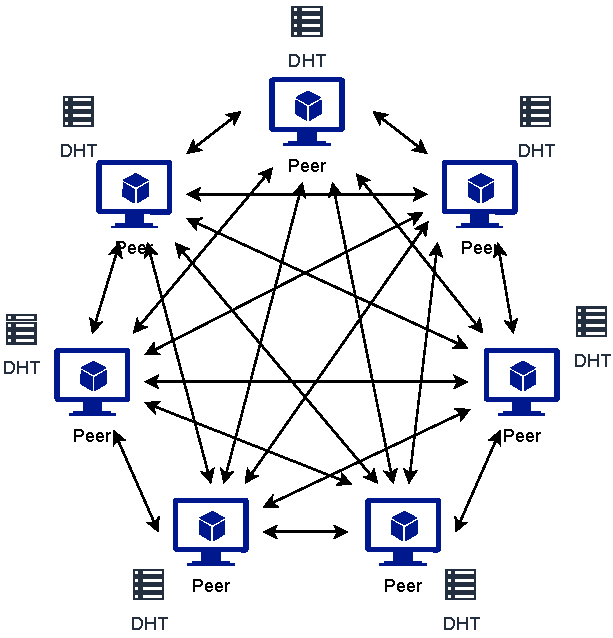
\includegraphics[width=0.5 \textwidth]{./figures/02_dht-communication.pdf}
\end{figure}

\subsection{Optimizer}
One of the main components of Hivemind is the Hivemind Optimizer, which wraps around any other implementation of a \texttt{torch.optim.Optimizer}.
Therefore, the Hivemind Optimizer can be used as a drop-in replacement in regular training operations.
With default settings and with no other peer, the Hivemind optimizer is designed to perform exactly as the underlying \texttt{torch.optim.Optimizer} class.
There are several options for tuning the Hivemind Optimizer, which affect how distributed training is performed across participating peers in a training run.
We will briefly describe some of the settings that we focused on during this thesis.

\subsubsection{Target Batch Size}

The target batch size (TBS) is defined in the Hivemind Optimizer as the global number of samples that every peer has collectively processed during a collaborative run in the current Hivemind epoch.
A Hivemind epoch, which we will call $HE$, does not necessarily correspond to a full pass over the training data and can be used to synchronize advanced training features like optimizer schedulers.
The HE starts at 0 at the beginning of training and increases by one every time that all participating peers reportedly finished processing $TBS$ since the last $HE$.

Understanding the concept of HE is crucial, so let us describe a simple scenario to aid with this task:
\begin{itemize}
    \item two peers are collaboratively training a model;
    \item the TBS is 256;
    \item the \texttt{use\_local\_updates} setting is set to \texttt{True} (see next section for a definition of this setting);
    \item each peer processes a batch size of 64;
    \item each peer processes every batch at roughly the same speed;
    \item each peer starts training at the same time.
\end{itemize}
After one step, the number of globally accumulated samples is equal to $64+64=128$, as each peer has processed the same amount of samples in the same amount of time.
After another step, the accumulated samples are equal to $128+(64+64)=256$.
Because the total number of accumulated samples is now 256 and it is equal to TBS, each peer can now initiate an averaging round with all other participating peers.
What happens right before and after averaging depends on the \texttt{use\_local\_updates} setting.

\subsection{Parameter Averaging}

Optimizers used for deep learning training such as SGD \cite{10.1214/aoms/1177729392} and ADAM \cite{10.48550/arxiv.1412.6980} need some information stored in memory to operate.
When training collaboratively, each peer may perform operations using a local version of these vectors to proceed with training.
However, optimizer parameters may diverge during training, in turn causing the underlying model parameters to diverge.
It is possible to mitigate this effect by performing operations that take into account all of the peer's information, for example with \textit{AllReduce} operations.
In the case of Hivemind, the operation of choice is averaging, which can be performed for both the optimizer state and the gradients before applying them to the model.

\begin{figure}[h]
    \centering
    \begin{subfigure}[b]{0.475 \textwidth}
        \centering
        \caption{}
        \label{fig:state-averaging}
        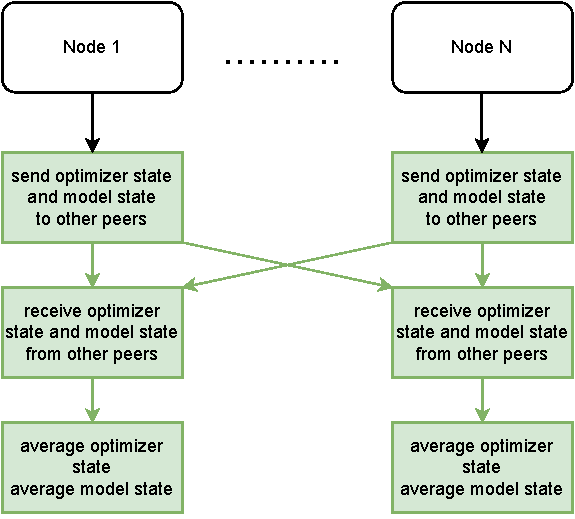
\includegraphics[width=\textwidth]{./figures/02_optimizer_averaging.pdf}
    \end{subfigure}%
    \hfill
    \begin{subfigure}[b]{0.475 \textwidth}
        \centering
        \caption{}
        \label{fig:gradient-averaging}
        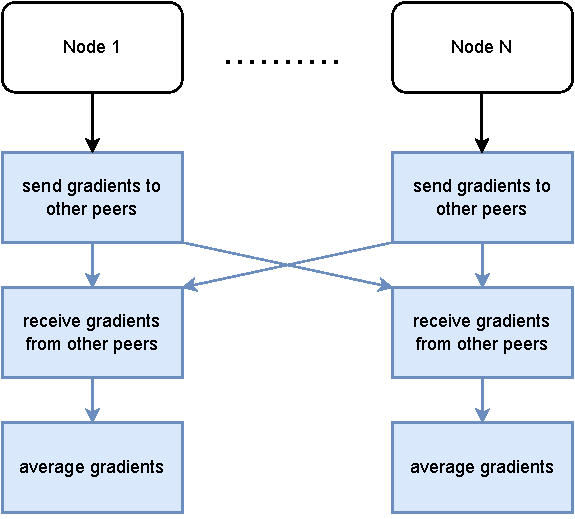
\includegraphics[width=\textwidth]{./figures/02_gradient_averaging.pdf}
    \end{subfigure}
    \caption{State averaging (left) and gradient averaging (right) in Hivemind.}
\end{figure}

\subsubsection{Local Updates}\label{ssec:local-updates}

Training neural networks with larger batches has been proven to be beneficial in some cases \cite{Krizhevsky2014owt, goyal2017accurate, you2017scaling}.
Thus, practitioners may want to be able to accumulate gradients either locally, in a distributed manner, or a combination of both.
Hivemind's implementation of distributed training extends the concept of gradient accumulation, previously presented in Subsection~\ref{sec:gradient-accumulation}, by introducing the \texttt{use\_local\_updates} settings for \texttt{hivemind.Optimizer}.

The setting has two modes:
\begin{itemize}
    \item \textbf{activated}; after every local training step, the Hivemind optimizer applies the gradients to the model.
          At the next HE, the final stage of the Optimizer starts.
          A simplified flow of how Hivemind implements this mode is illustrated in \autoref{fig:use-local-updates_true}.
    \item \textbf{deactivated}; after every local training step, gradients are accumulated instead of being applied to the model's parameters.
          After $ACC$ steps, the optimizer is invoked and internally stores the accumulated gradients.
          At the next HE, the Optimizer averages the accumulated gradients with all participating peers.
          The final stage of the Optimizer then starts, which averages the model and optimizer state with other peers.
          A simplified flow of how Hivemind implements this mode is illustrated in \autoref{fig:use-local-updates_false}.
\end{itemize}

\begin{figure}[h]
    \centering
    \caption{Diagram of Hivemind training with local updates enabled.}
    \label{fig:use-local-updates_true}
    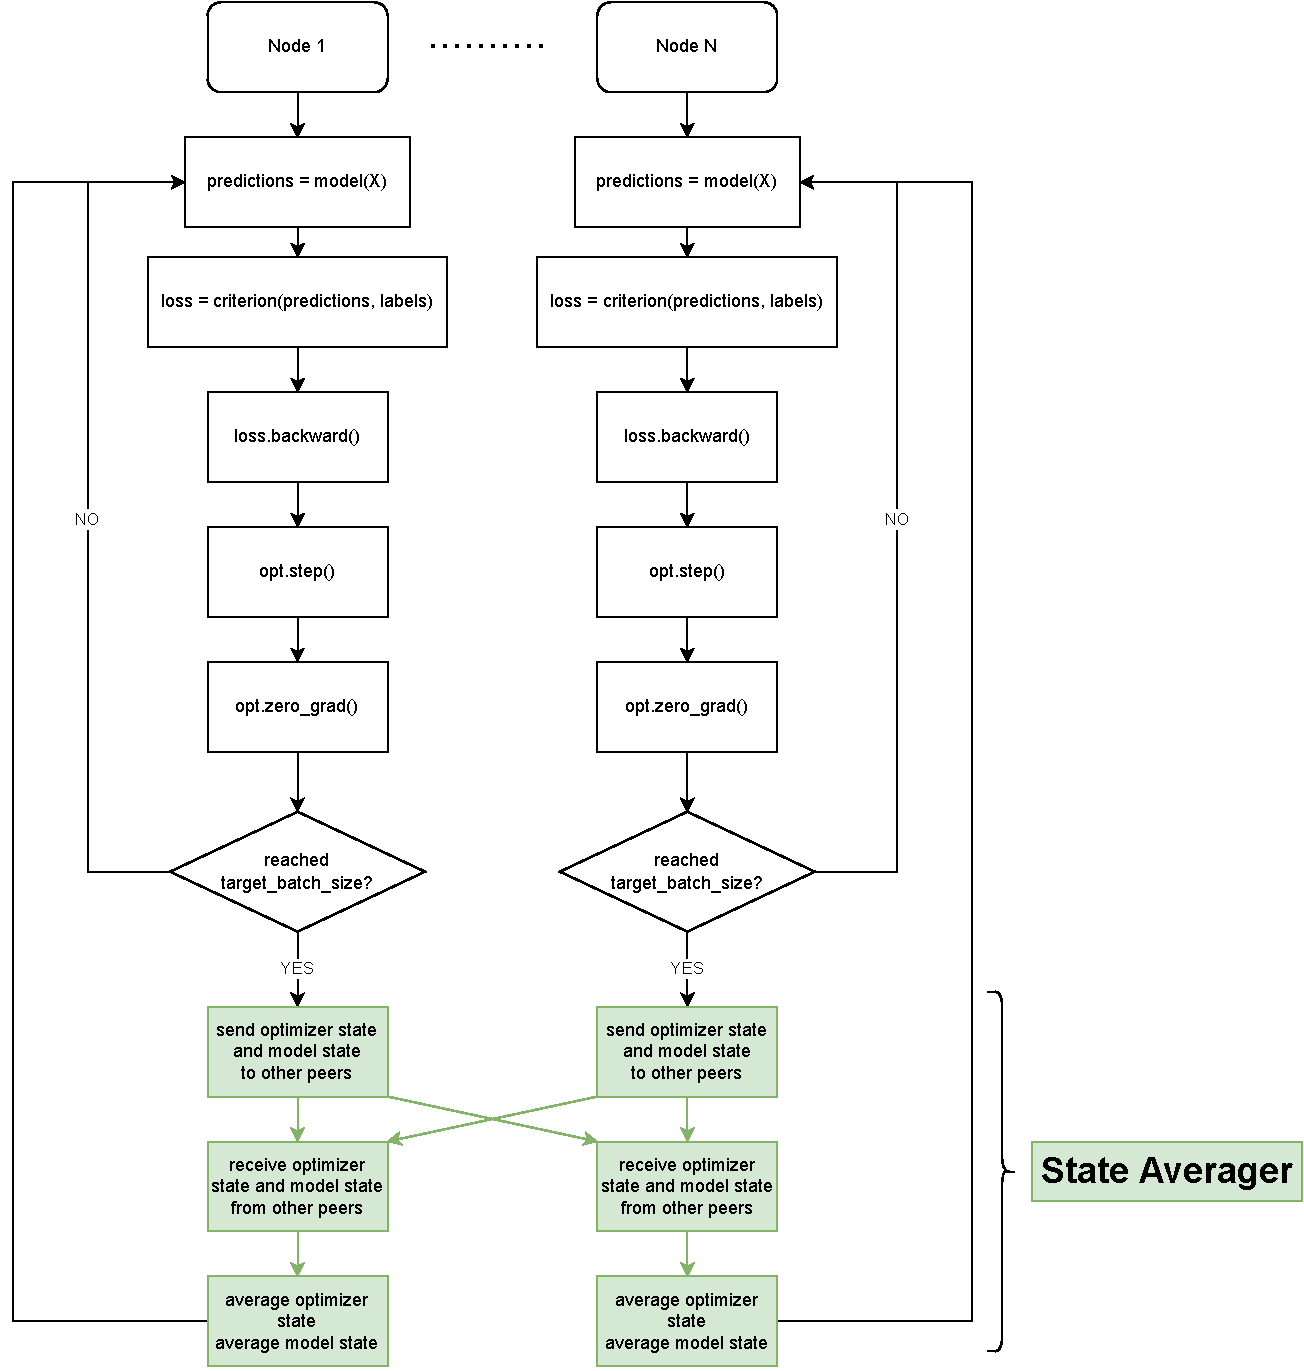
\includegraphics[width=0.8 \textwidth]{./figures/02_use-local-updates_true.pdf}
\end{figure}

\begin{figure}[h]
    \centering
    \caption{Diagram of Hivemind training with local updates disabled.}
    \label{fig:use-local-updates_false}
    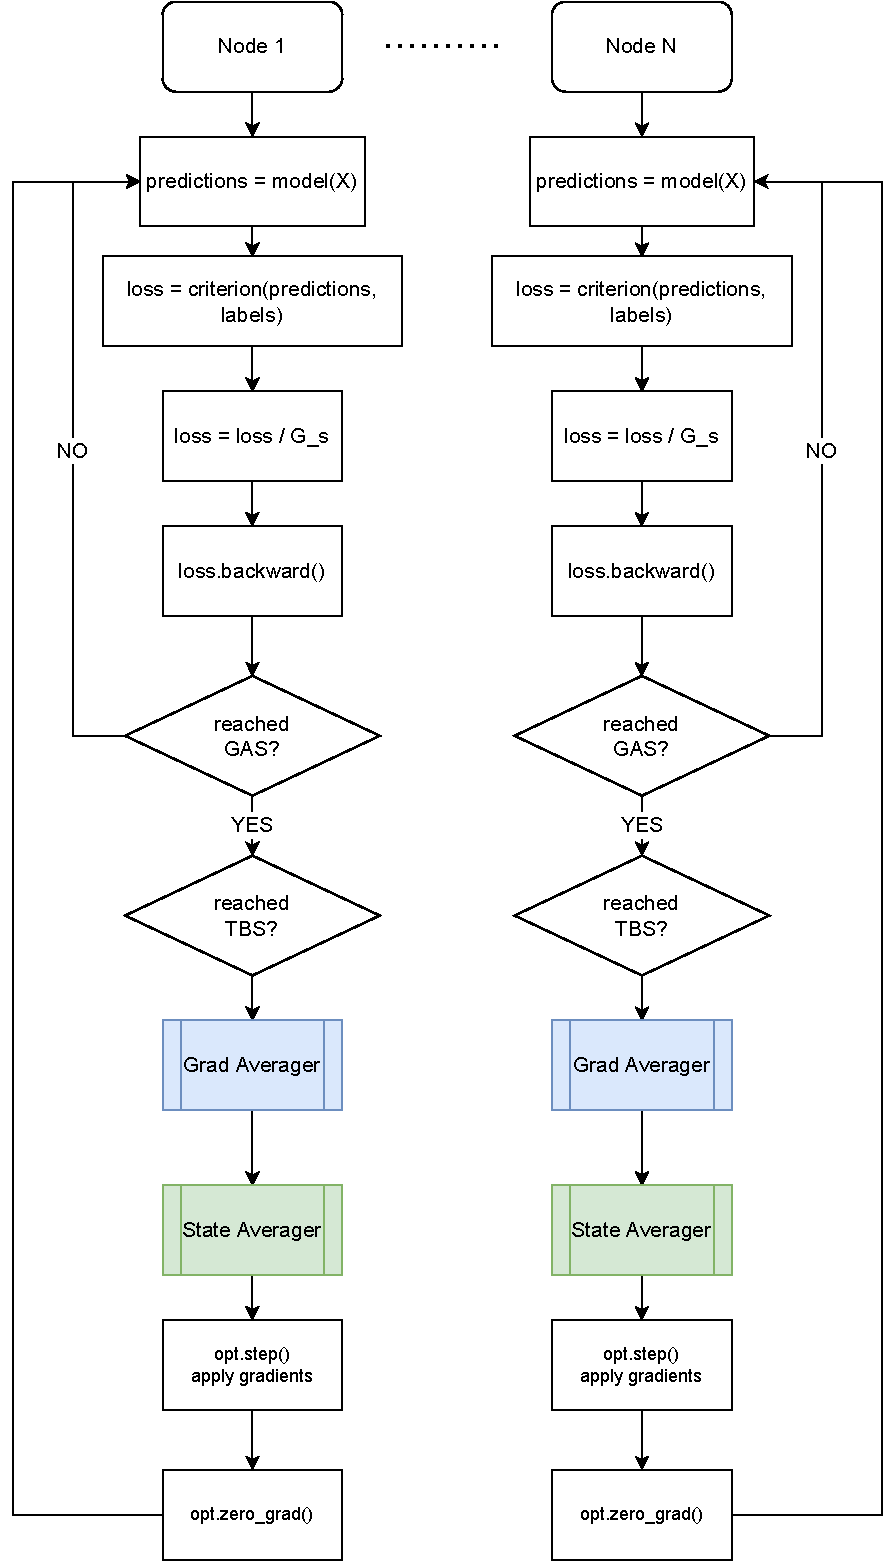
\includegraphics[width=0.7 \textwidth]{./figures/02_use-local-updates_false.pdf}
\end{figure}


In this thesis, we will discuss the effects of enabling or disabling this setting on training.
